\section{Introduction}
%(2 pages)}
\label{sec:intro}

\leanparagraph{Motivation}
Recent advances in information extraction have led to
huge graph-structured knowledge bases (KBs) also known as knowledge graphs (KGs) such as NELL \cite{nell}, DBpedia \cite{dbpedia}, YAGO \cite{yago} and Wikidata \cite{wikidata}. These KGs contain millions or billions of relational facts in the form of subject-predicate-object (SPO) triples, e.g., $\tuple{\mi{clara\;isMarriedTo\;dave}}$ or $\tuple{\mi{dave\;isA\;researcher}}$. 

An important task over KGs is rule learning, which is relevant for a variety of applications ranging from knowledge graph curation (completion, error detection) \cite{DBLP:journals/semweb/Paulheim17} to data mining and semantic culturonomics. 
Traditionally, rule extraction has been studied in the context of relational data mining (see e.g., \cite{amie,op,rdf2rules}). These methods can be used to identify prominent patterns, such as \emph{``Married people live in the same
place''}, and cast them in the form of Horn rules, such as:
$\mi{r_1:\;}\mi{livesIn(Y,Z)}\leftarrow \mi{isMarriedTo(X,Y),livesIn(X,Z)}$.

For the KG curation, this has twofold benefits. First, since KGs operate under the Open World
Assumption (OWA) (i.e., absent facts are treated as unknown rather than false),
the rules can be used to derive additional facts. For example, applying the rule
$\mi{r_1}$ mined from the graph in Figure~\ref{rdf}, the missing living place of Dave can be deduced based on the data about his wife Clara. Second, rules can be used to eliminate erroneous facts in the KG. For example, assuming
that $\mi{livesIn}$ is a functional relation, Amsterdam as a living place of
Alice could be questioned as it differs from her husband's.

Horn rules such as $r_1$, where all predicates in the rule body are positive,  might not always be sufficiently expressive % .
% This is insufficient
to capture KG patterns accurately. Indeed, Horn rules cannot handle exceptions, which often appear in practical applications, and thus such rules might make incorrect predictions on missing facts.
For example, consider a more accurae version of $\mi{r_1}$ given as \\$\mi{r_2{:}livesIn(Y,Z){\leftarrow}
  isMarriedTo(X,Y){,}livesIn(X,Z){,}{\naf\,} researcher(Y)}$, which \\states that \emph{``Married people live in the same place unless one is a
  researcher''}. The additional knowledge that Alice is a researcher could be actually an explanation for her living in an unexpected place. If $\mi{r_2}$ often holds, then
one can no longer complete the missing living place for Dave by assuming that he lives with his wife Clara. 
Understanding exceptions is crucial for KG completion and curation, and it has been therefore studied in several recent works \cite{DBLP:conf/semweb/Gad-ElrabSUW16,rumis}.

Particularly challenging property of KGs for extraction of meaningful rules is their incompleteness and strong data bias. 
Indeed, rules learned from incomplete KGs might be erroneous and might make incorrect predictions on missing facts. 
For example, $\mi{r_3}: \mathit{hasChild(X,Y)}\leftarrow \mathit{worksAt}(X,Z),\mathit{educatedAt}(Y,Z)$ could be mined from a highly incomplete and biased KG stating that workers of certain institutions often have children among the people educated there, 
as this is frequently the case for popular scientists.

Recently, efforts have been put into detecting the concrete numbers of 
facts of certain types that hold in the real world 
(e.g., \emph{``Einstein has 3 children''}) by exploiting Web extraction and crowd-sourcing methods~\cite{cardinality-extraction-iswc-2016,cool-wd}. Such 
meta-data provides a lot of hints about the topology of KGs, and reveals 
parts that should be especially targeted by rule learning methods.
This additional knowledge can be effectively exploited in the rule learning process as shown in \cite{carl}.



The aim of this article is to survey the current research on rule learning from knowledge graphs. We present and discuss different techniques with the roots in inductive logic programming and relational data mining as well as their interalation and applications for KGs. 

\leanparagraph{Overview}


\begin{figure}[t]
\centering
\begin{subfigure}[b]{0.75\textwidth}
    \centering
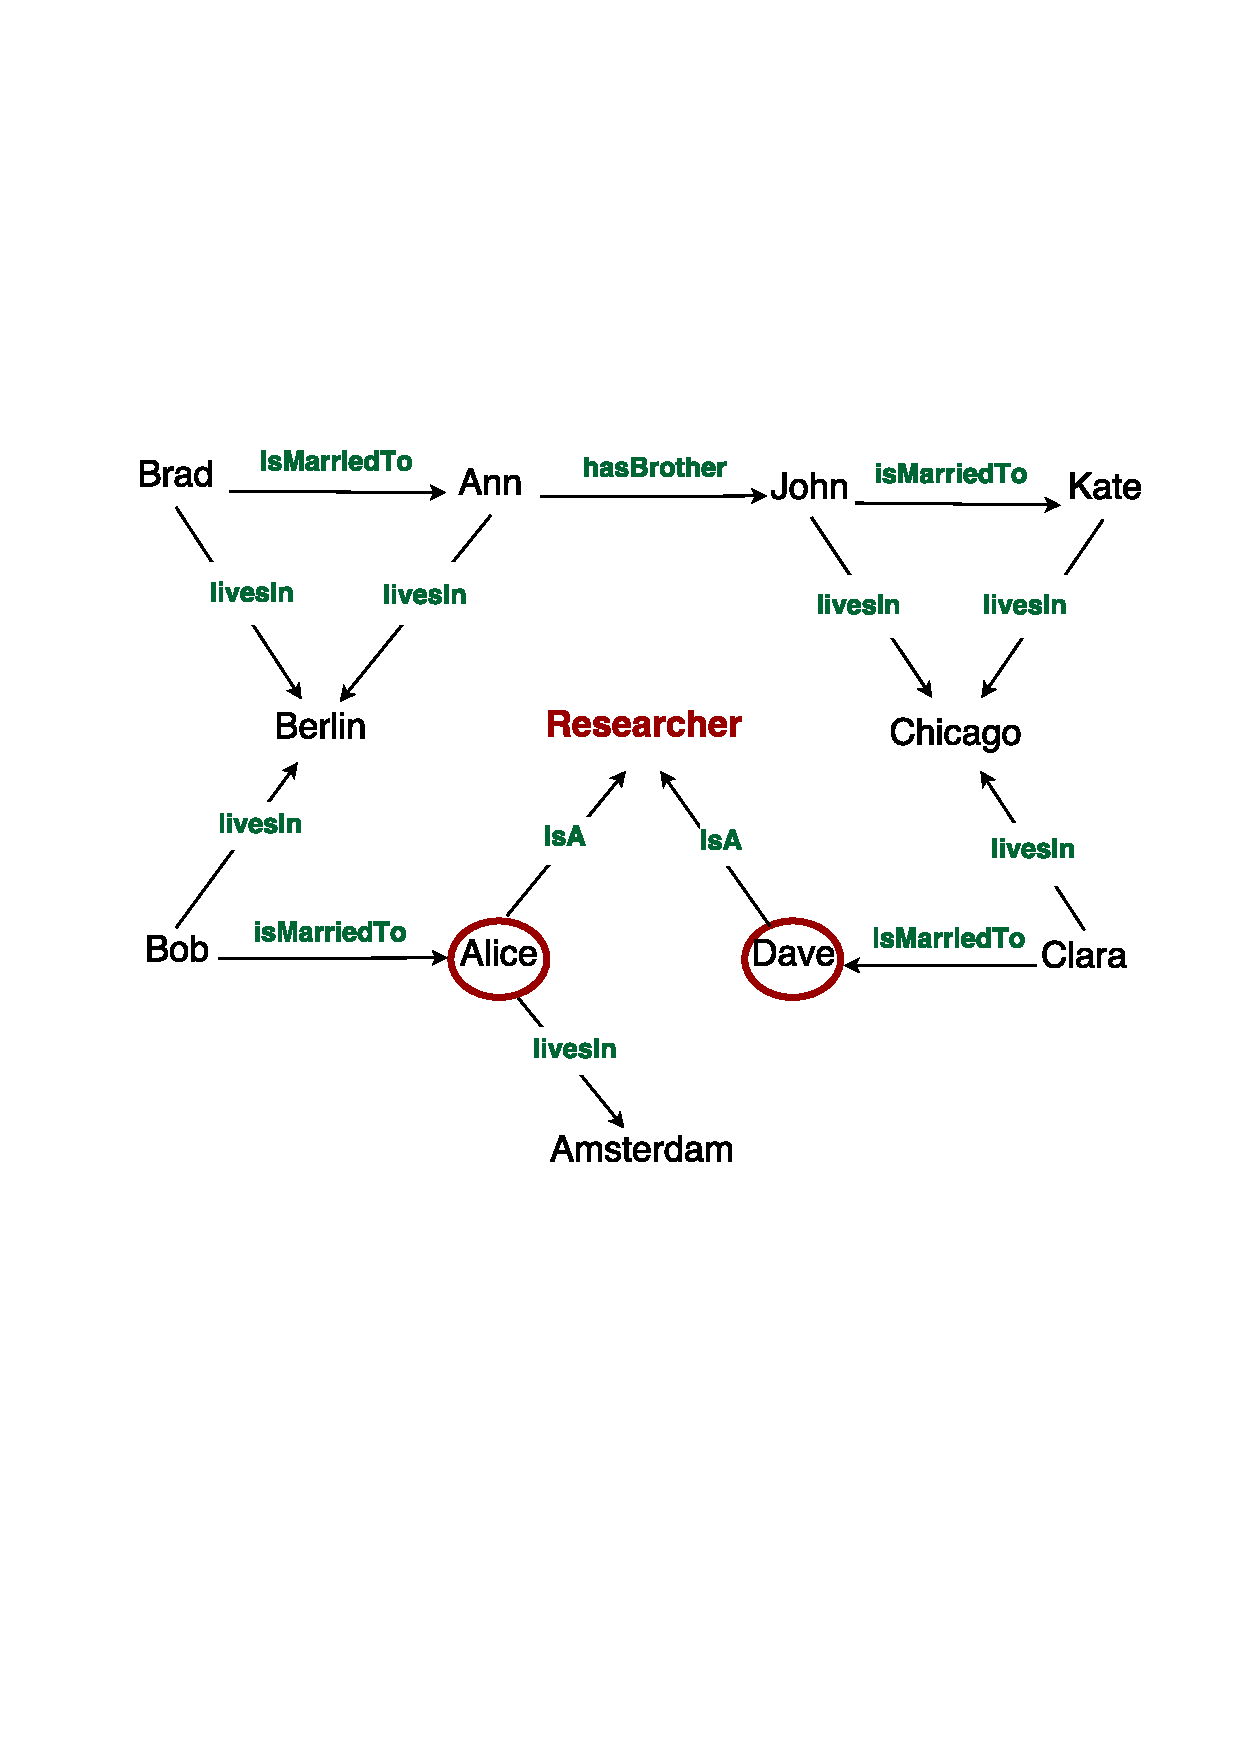
\includegraphics[width=0.7\textwidth]{figures/kg}
\caption{Rule mining for KG completion and KG cleaning}
\label{rdf}
\end{subfigure}
\begin{subfigure}[b]{0.24\textwidth}
\scriptsize
\renewcommand*{\arraystretch}{0.95}
\begin{tabular}{|l|l|l|l|l|l|l|l|l|}
\hline
&  \rot{$\mi{bornInUS}$} &\rot{$\mi{livesInUS}$}&
\rot{$\mi{stateless}$}&\rot{$\mi{immigrant}$}&\rot{$\mi{singer}$}&\rot{$\mi{poet}$}&\rot{$\mi{hasUSPass}$}\\ \hline
$\mi{p1}$ & $\checkmark$ &$\checkmark$ &&&$\checkmark$&&$\checkmark$ \\ \hline
$\mi{p2}$ & $\checkmark$ &$\checkmark$ &&&&&$\checkmark$ \\ \hline
$\mi{p3}$ & $\checkmark$ &$\checkmark$ &&&$\checkmark$&$\checkmark$&$\checkmark$ \\ \hline
$\mi{p4}$ & $\checkmark$ &$\checkmark$ &&&&&$\checkmark$ \\ \hline
$\mi{p5}$ & $\checkmark$ &$\checkmark$ &$\checkmark$&&&& \\ \hline
$\mi{p6}$ & $\checkmark$ & &$\checkmark$&&&& \\ \hline
$\mi{p7}$ & $\checkmark$ & &$\checkmark$&&&& \\ \hline
$\mi{p8}$ & $\checkmark$ & &$\checkmark$&$\checkmark$&&& \\ \hline
$\mi{p9}$ & $\checkmark$ & &&$\checkmark$&&$\checkmark$& \\ \hline
$\mi{p10}$ & $\checkmark$ & &&$\checkmark$&$\checkmark$&$\checkmark$& \\ \hline
$\mi{p11}$ & $\checkmark$ & &&&$\checkmark$&$\checkmark$&$\checkmark$ \\ \hline
\end{tabular}
\smallskip
\caption{US inhabitants KG}
\label{tab:im}
\end{subfigure}
\caption{Examples of Knowledge Graphs}
\end{figure}



\begin{figure}[t]
\begin{center}
%\includegraphics[width=.8\textwidth]{figures/fam_grad}

%%%%%% New KG %%%%%%%

\begin{tikzpicture}[->,>=stealth',auto,node distance=3cm,
  thick,main node/.style={font=\bfseries}]

  \node[main node] (1) {john};
  \node[main node] (2) [right=3cm of 1] {mary};
  \node[main node] (3) [below left=1cm and 2cm of 1] {alice};
  \node[main node] (4) [below right=1cm and 1.5cm of 1] {bob};
  \node[main node] (5) [below right=1cm and 2cm of 2] {carol};
  \node[main node] (6) [above left=1cm and 2cm of 1] {dave};
  \node[main node] (7) [above right=1cm and 1.5cm of 1] {tuwien};
  \node[main node] (8) [above right=1cm and 2cm of 2] {mpi};

  \path[every node/.style={color=teal,fill=white,font=\small}]
    (1) edge node [right=-20pt] {worksAt} (7)
    (2) edge node [right=-15pt] {worksAt} (7)
    (4) edge node [right=-30pt] {educatedAt} (7)
    (2) edge node [right=-10pt] {hasChild} (4)
    (2) edge node [left=-20pt] {hasChild} (5)
    (1) edge[bend left=20] node [right=-20pt] {hasChild} (4)
    (4) edge[bend left=20] node [left=-20pt] {hasFather} (1)
    (1) edge[bend right=20] node [right=-20pt] {hasChild} (3)
    (3) edge[bend right=20] node [right=-20pt] {hasFather} (1)
    (2) edge node [left=-20pt] {educatedAt} (8)
    (5) edge[bend left=20] node [left=-10pt] {educatedAt} (8)
    (5) edge[bend right=20] node [right=-10pt,pos=0.4] {worksAt} (8)
    (6) edge node [right=-5pt] {hasFather} (1)
    (3) edge[bend right=20] node [right=-10pt,pos=0.55] {hasSibling} (6)
    (6) edge[bend right=20] node [left=-10pt,pos=0.65] {hasSibling} (3)
    (6) edge[bend left=20] node [above=-10pt] {worksAt} (7)
    (6) edge[bend right=5] node [below=-10pt] {educatedAt} (7)
    (4) edge node [right=-20pt] {hasSibling} (5)
    ;
\end{tikzpicture}

\caption{Example KG}
\label{fig:fam_grad}
\end{center}
\end{figure}